%%
%% VERSION HISTORY
%%    22 May 2006 - John Papandriopoulos - Original version
%%    12 Jul 2007 - John Papandriopoulos - Converted into template
%%

\chapter[Appendix]{Computation of the articular deceleration capabilities for a robotic manipulator}
\label{app:constrcomp}
\setfigurepath{figures/Constrcomp}
For a robotic manipulator, the relation between the control torque input $\vect{\tau}_{|k}^c$ and the resulting articular acceleration $\vect{\ddot{q}_{|k}}$ can be expressed using the equations corresponding to its dynamic model: 
\begin{equation}
M(\vect{q}_{|k}) \vect{\ddot{q}}_{|k} + \vect{b}(\vect{q}_{|k},\vect{\dot{q}}_{|k}) = \vect{\tau}_{|k}^c.
\label{eq:dyn_eq_bis}
\end{equation}
Therefore, the maximum producible deceleration/acceleration $[\boldsymbol{\ddot{q}}_m, \boldsymbol{\ddot{q}}_M]$ is function of the minimum and maximum producible torque $[\vect{\tau}_m, \vect{\tau}_M]$ (usually specified by the system's manufacturer) in addition to the instantaneous state $\{\vect{q}_{|k},\vect{\dot{q}}_{|k}\}$ of the system. Instantaneous  minimum and maximum producible decelerations $(\vect{\ddot{q}}_{m}^{~inst}, \vect{\ddot{q}}_{M}^{~inst})$ can be computed:
\begin{gather}
\argmin \limits_{\boldsymbol{\tau}_{|k}} \boldsymbol{M}(\vect{q}_{|k})^{-1} (\vect{\tau}_{|k}-\vect{b}(\vect{q}_{|k},\vect{\dot{q}}_{|k})),
\raisetag{-.5em}
\label{eq:qddot_minimizing_opt_1}
\end{gather}
\begin{gather}
\argmax \limits_{\boldsymbol{\tau}_{|k}} \boldsymbol{M}(\vect{q}_{|k})^{-1} (\vect{\tau}_{|k}-\vect{b}(\vect{q}_{|k},\vect{\dot{q}}_{|k})),
\raisetag{-.5em}
\label{eq:qddot_maximizing_opt_2}
\end{gather}
s.t: $\vect{\tau}_m \leq \vect{\tau}_{|k} \leq \vect{\tau}_M$ \\
Then: 
\begin{equation}
\vect{\ddot{q}}_{M}^{~inst} =  \boldsymbol{M}(\vect{q}_{|k})^{-1} (\vect{\tau}_{max}-\vect{b}(\vect{q}_{|k},\vect{\dot{q}}_{|k})), 
\label{eq:qddot_maximizing}
\end{equation}
\begin{equation}
\vect{\ddot{q}}_{m}^{~inst} =  \boldsymbol{M}(\vect{q}_{|k})^{-1} (\vect{\tau}_{min}-\vect{b}(\vect{q}_{|k},\vect{\dot{q}}_{|k})), 
\label{eq:qddot_minimizing}
\end{equation}
where $\vect{\tau}_{min}$ and $\vect{\tau}_{max}$ are respectively the instantaneous solutions for (\ref{eq:qddot_minimizing_opt_1}) and (\ref{eq:qddot_maximizing_opt_2}) during the movement of the robot shown in Fig.~\ref{fig:kuka_screen}. Note that these two parameters differ from  $\vect{\tau}_{m}$ and $\vect{\tau}_{M}$, as $\vect{\tau}_{m}$ and $\vect{\tau}_{M}$ do not obligatory generate the maximum positive and negative producible articular decelerations.\\
For a KUKA LWR4 serial robot with: $\vect{\tau}_{M}^{T} = -\vect{\tau}_{m}^{T} = [200,\allowbreak 200,\allowbreak 100,\allowbreak 100,\allowbreak 100,\allowbreak 30,\allowbreak 30]$, the instantaneous maximum and minimum producible accelerations for joint $0$ during the movement shown in Fig.~\ref{fig:kuka_screen} are depicted in Fig.~\ref{fig:instant_articular_acceleration_capability}. 
\begin{figure*}
\centering
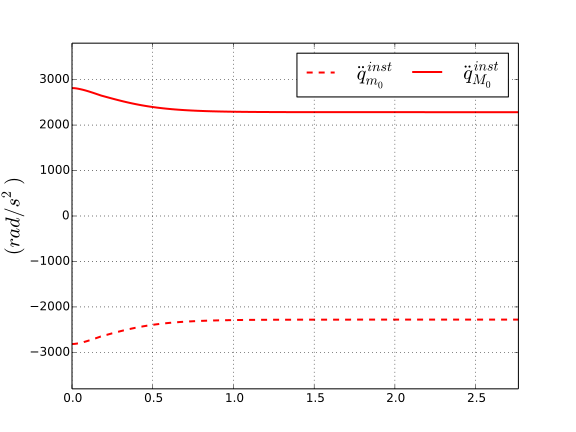
\includegraphics[width=0.8\columnwidth]{/home/anis/Desktop/THESIS_ANIS/THESIS1/figures/Constrcomp/instant_articular_acceleration_capability}
\caption{Instantaneous producible maximum and minimum articular accelerations for joint $0$ during the movement of the KUKA LWR4 as shown in Fig.~\ref{fig:kuka_screen}.}
\label{fig:instant_articular_acceleration_capability}
\end{figure*}\\
However, as  $\boldsymbol{\ddot{q}}_M$ and $\boldsymbol{\ddot{q}}_m$ are used as constants in the formulation of the constraints on articular velocity and position, the final values for these parameters can be computed using algorithm~\ref{alg:compute_q_ddot_m_q_ddot_M} :
\begin{algorithm}
\caption{Compute $\boldsymbol{\ddot{q}}_M$ and $\boldsymbol{\ddot{q}}_m$}
\label{alg:compute_q_ddot_m_q_ddot_M}
\begin{algorithmic}[1]
\Require $\vect{q}_M, \vect{q}_m, \vect{\dot{q}}_{M},\vect{\dot{q}}_{m}, \vect{\tau}_m, \vect{\tau}_M, N$
\myState{$\vect{\ddot{q}}_{m} \gets -[\infty,...,\infty]$} 
\myState{$\vect{\ddot{q}}_{M} \gets [\infty,...,\infty]$} 
\For{($i = 1 \rightarrow N$)}
        \myState{$\vect{q} \gets random(\vect{q}_{m}, \vect{q}_{M})$}
        \myState{$\vect{\dot{q}} \gets random(\vect{\dot{q}}_{m}, \vect{\dot{q}}_{M})$}
        \myState{compute $\vect{\tau}_{max}$ & $\vect{\tau}_{min}$ using (\ref{eq:qddot_minimizing_opt_1}) and (\ref{eq:qddot_minimizing_opt_1})}
        \myState{$\boldsymbol{\ddot{q}}_M^{~inst} \gets M(\vect{q})^{-1}(\vect{\tau}_{max}-b(\vect{q}, \vect{\dot{q}}))$}
        \myState{$\boldsymbol{\ddot{q}}_m^{~inst} \gets M(\vect{q})^{-1}(\vect{\tau}_{min}-b(\vect{q}, \vect{\dot{q}}))$}
        \If{($\vect{\ddot{q}}_{M}^{~inst} \leq \vect{\ddot{q}}_{M}$)}
            \State{$\vect{\ddot{q}}_{M} \gets \vect{\ddot{q}}_{M}^{~inst}$}
        \EndIf 
                \If{($\vect{\ddot{q}}_{m}^{~inst} \geq \vect{\ddot{q}}_{m}$)}
            \State{$\vect{\ddot{q}}_{m} \gets \vect{\ddot{q}}_{m}^{~inst}$}
        \EndIf             
\EndFor
\myState \Return{$\vect{\ddot{q}}_{M}, \vect{\ddot{q}}_{m}$}\;
\end{algorithmic}
\end{algorithm}

          
%       
%Let $q(k), \dot{q}(k), \ddot{q}(k)$ and $\dddot{q}(k)$ be the sequences of joint positions, velocities, accelerations and jerk. In discrete time, the motion is modelized by: 
%
%\begin{equation} 
%\left\{\begin{array}{lcl}
%\vect{q}(k+1) = \vect{q}(k) + \vect{\dot{q}}(k) \delta t, \\
%\vect{\dot{q}}(k+1) = \vect{\dot{q}}(k) + \vect{\ddot{q}}(k) \delta t, \\
%\vect{\ddot{q}}(k+1) = \vect{\ddot{q}}(k) + \vect{\dddot{q}}(k) \delta t.
%\end{array}\right.
%\label{eq:discretized_dynamics}
%\end{equation}
%
%\subsection{Joint jerk and velocity limits}
%In case of constant jerk, the evolution of joint velocity in $n_1$ time steps is :
%
%
%If we suppose $\dot{q}(k) > 0$ and $\dddot{q}_m < 0$ (negative jerk example), the condition $\dot{q}(k+n_1) \leq \dot{q}_M$ for all integer $n_1$ leads to :
%
%\begin{equation}
%\begin{split}
%\ddot{q}(k) \leq \frac{\dot{q}_M-\dot{q}(k)}{n_1 \delta t} - \frac{(n_1-1)}{2} \dddot{q}_m \delta t 
%\label{eq:q_ddot_vel_jerk_comp}
%\end{split}
%\end{equation}
%
%Where $n_1$, the integer minimizing the right hand side of (\ref{eq:q_ddot_vel_jerk_comp}). By diferentiating this expression w.r.t $n_1$ :
%
%\begin{equation} 
%\left. \begin{array}{r} 
%n_1 \geq 1 \\
%\frac{-(\dot{q}_M-\dot{q}(k))}{n_1^2 \delta t} - \frac{1}{2} \dddot{q}_m \delta t = 0
%\end{array} \right\} 
%\Leftrightarrow n_1=-\frac{\sqrt{-2\dddot{q}_m(\dot{q}_M-\dot{q}(k))}}{\dddot{q}_m \delta t}
%\label{eq:n_1_eq}
%\end{equation}
%
%$n_1$ must be $\geq 1$ so the acceleration constraint is not violated. Moreover, the presented method may fail in case of any measurements errors. 
%
%\subsection{Joint acceleration and position limits}
%As shown in \cite{decre2009extending}, in case of constant acceleration $\ddot{q}_m$, the evolution of the position in $n_3$ iterations is : 
%
%\begin{equation}
%\begin{split}
%q(k+n_3)=q(k)+n_3 \dot{q}(k) \delta t +  \frac{(n_3^2-n_3)}{2} \ddot{q}_m \delta t^2
%\label{eq:q_evolution_with_const_qddot_m}
%\end{split}
%\end{equation}
%
%If we suppose $\dot{q}(k) > 0$ and $\ddot{q}_m < 0$ (deceleration example), the condition $q(k+n_3) \leq q_M$ for all integer $n_3$ leads to : 
%
%\begin{equation}
%\begin{split}
%\dot{q}(k) \leq \frac{q_M-q(k)}{n_3 \delta t} - \frac{(n_3-1)}{2} \ddot{q}_m \delta t
%\label{eq:q_dot_posi_acc_comp}
%\end{split}
%\end{equation}
%
%Which is written on the dynamic level : 
%
%\begin{equation}
%\begin{split}
%\ddot{q}(k) \leq \frac{q_M-q(k+1)}{n_3 \delta t^2} - \frac{(n_3-1)}{2} \ddot{q}_m - \frac{\dot{q}(k)}{\delta t}
%\label{eq:q_ddot_posi_acc_comp}
%\end{split}
%\end{equation}
%
%With : $q(k+1) = q(k)+\dot{q}(k) \delta t$, an overestimation \footnote{ Because it is computed during a braking phase, the estimation of the position for the next time step will always be less than the real position : $q_{estimated}(k+1) \leq q_{real}(k+1)$} of the actuator position at the next time step.
%
%$n_3$ is the integer minimizing the right hand side of (\ref{eq:q_dot_posi_acc_comp}). By differentiating this expression w.r.t $n_3$ :
%
%\begin{equation} 
%\left. \begin{array}{r} 
%n_3 \geq 1 \\
%\frac{-(q_M-q(k))}{n_3^2 \delta t} - \frac{1}{2} \ddot{q}_m \delta t= 0
%\end{array} \right\} 
%\Leftrightarrow n_3=-\frac{\sqrt{-2\ddot{q}_m(q_M-q(k))}}{\ddot{q}_m \delta t}
%\label{eq:n_3_eq}
%\end{equation}
%
%\subsection{Joint jerk and position limits}
%In case of constant jerk $\dddot{q}_m$, the position evolution in $n_5$ iterations is :
%
%If we suppose $\dot{q}(k) > 0$ and $\dddot{q}_m < 0$ (negative jerk example), the condition $q(k+n_5) \leq q_M$ for all integer $n_5$ leads to : 
%
%\begin{equation}
%\begin{split}
%\ddot{q}(k) \leq \frac{2(q_M-q(k))}{(n_5^2-n_5) \delta t^2} - \frac{2 \dot{q}(k)}{(n_5-1) \delta t} - \frac{(\frac{n_5^2}{3}-n_5+\frac{2}{3})\ddot{q}_m \delta t}{(n_5-1)} 
%\label{eq:q_ddot_posi_jerk_comp}
%\end{split}
%\end{equation}
%
%$n_5$ is the integer minimizing the right hand side of (\ref{eq:q_ddot_posi_jerk_comp}). By differentiating this expression w.r.t $n_5$ :
%
%\begin{equation}
%\left\{\begin{array}{lcl}
%n_5 \geq 3 \\
%\begin{split}
%-&(\frac{1}{3} \dddot{q}_m(k) \delta t^3) n_5^4 + (\frac{2}{3} \ddot{q}(k) \delta t^3) n_5^3  \\
%+&(2 \dot{q}(k) \delta t - \frac{1}{3} \dddot{q}_m(k) \delta t^3) n_5^2 \\
%+&(4 (q_M-q(k)) n_5 - 2(q_M-q(k)=0
%\end{split}
%\end{array}\right.
%\label{eq:n_5_eq}
%\end{equation}
%
%Indeed, $n_5$ must be $\geq 3$ so $\dddot{q}_m$ is always part of (\ref{eq:q_ddot_posi_jerk_comp}). 
